\documentclass[a4paper]{article}

\usepackage[a4paper]{geometry}
\usepackage{amssymb,amsmath}
\usepackage[utf8]{inputenc}
\usepackage{enumerate}
\usepackage{color}
\usepackage{graphicx}
\usepackage[estonian]{babel}
\usepackage[usenames,dvipsnames]{xcolor}
\usepackage{float}
\usepackage{cite}
\usepackage{etoolbox}
\usepackage[hidelinks]{hyperref}

\allowdisplaybreaks
\makeatletter
\patchcmd{\HyField@FlagsRadioButton}{\HyField@SetFlag{Ff}{Radio}}{}{}{}
\makeatother
\def\DefaultOptionsofRadio{print}



\definecolor{background_example}{HTML}{E0DCDE}



\setlength\parindent{0pt}
\newenvironment{tightcenter}{%
  \setlength\topsep{0pt}
  \setlength\parskip{0pt}
  \begin{center}
}{%
  \end{center}
}

\author{Vootele Rõtov}
\title{Bakatöö}
\begin{document}

\maketitle

\pagebreak

\tableofcontents

\pagebreak

\section*{Spikker}

{\color{cyan} Helesinine- komentaarid}

{\color{blue} Tumesinine - asjad, mille õigsust peaks kontrollima}


{\color{cyan}\section*{Miks ma käesolevat asja teen?}

Panen kirja mõned põhjused, miks ma tegelen selle asjaga:
\begin{enumerate}[I]
\item Sellest on kellegile kasu - loodan realselt, et saan hakkama mingi toreda asjaga, millest keegi(näiteks Marguse psühholoogidest sõbrad) kasu saab.
\item Saab kätte selle paberi, mis teeb minust parema inimese. 
\item Midagi uut, olen juba päris pikalt tarkust ühes formaadis kuula õppejõudu, tööta läbi tema poolt valitud materjalid, esita see õppejõule, äkki selline formaat, kus tuleb ise otsida ja ise mõelda meeldib.
\item Väljakutse, kuigi viimaste aastatega on enesemotivatsioon kõvasti paranenud, ei ole see veel seal, kus ta olla võiks. Loodetavasti "treenin" seda aspekti.
\end{enumerate}}

\section{Töö \"ulesehitus}
Esiteks, toome sisse lugejale vajaliku taustinfo, seejärel kirjeldame probleemip\"ustitust. Sellele järgneb töö eesmärgi matemaatiline p\"ustitus.

\section{Taustinfo}

\subsection{Likerti skaala
}
Käesolev uurimus tegeleb k\"usimustikega (\textit{Likert scale}), milles soovitakse hinnanguid mingile arvule väidetele (\textit{Likert item}) viie pallisel Likerti skaalal.\cite{Edmondson} Näiteks: \footnote{Näited terviklikest k\"usimustikest lisades, \hyperref[likert1]{joonis \ref*{likert1}} ja \hyperref[likert2]{joonis \ref*{likert2}}}

\vspace{10pt}

\begin{figure}[H]


\colorbox{background_example}{\parbox{\textwidth}{

\vspace{1mm}

Käesoleva bakalaureusetöö \"ulesehitus on loogiline.

\vspace{5pt}

\begin{Form}
\def\DefaultWidthofChoiceMenu{12pt}%



\ChoiceMenu[bordercolor = gray,disabled = true,name=optionE,radio,radiosymbol=\ding{108}]{\mbox{}}\null Ei nõustu 
\ChoiceMenu[bordercolor = gray,disabled = true,name=optionD,radio,radiosymbol=\ding{108}]{\mbox{}}\null Ei nõustu osaliselt
\ChoiceMenu[bordercolor = gray,disabled = true,name=optionC,radio,radiosymbol=\ding{108}]{\mbox{}}\null Nii ja naa
\ChoiceMenu[bordercolor = gray,disabled = true, name=optionB,radio,radiosymbol=\ding{108}]{\mbox{}}\null Nõustun osaliselt
\ChoiceMenu[bordercolor = gray,disabled = true,name=optionA,radio,radiosymbol=\ding{108}]{\mbox{}}\null Nõustun


\end{Form}}}
\caption{Näide väitest, millele palutakse hinnangut Likerti skaalal}
\label{likert_question}
\end{figure}

\paragraph{Likerti skaala -  järjestikskaala või intervallskaala?}\mbox{}\\*

Lugejal võib tekkida õigustatud k\"usimus, kuidas põhjendab autor Likerti skaala käsitlemist intervall kui Likerti skaala oli algselt mõeldud järjestikskaalana ning  selle kasutamise osas intervallskaalana on autorid pigem skeptilised. \cite{Jamieson2004} Autori ei tunne ennast pädevana otsustamaks, kas Likerti skaala selline tõlgendamine on õigustatud, k\"ull aga on praktitkas selline tõlgendus piisavalt levinud, et selle valdkonna uurimine õigustatud oleks. Siinkohal märgin ära, et kriitikute \"uks levinumaid argumente on see, et "hea" ja "väga hea" keskmine ei ole mingil loomulikul viisil tõlgendatav kui  "hea + pool", millega autor nõustub ning loodab pakuda sellele alternatiivset tõlgendust. 

\subsection{Reliaablus}
Testi reliaabluseks nimetatakse testi omadust saada sama subjekti erinevatel mõõtmistel sama tulemus. Kõrge reliaablusega testi tulemuste juhuslik viga on väike. Järgnev joonis illustreerib reliaabluse konseptsiooni, suhestades teda teiste testi karakteristiku, valiidsusega.

\begin{figure}[H]
\centering

\includegraphics[width=0.75\textwidth, height = 0.8\textwidth]{Reliability_and_validity.png}
\caption{Reliaabluse (\textit{reliability}) ja valiidsuse (\textit{validity}) omavahelist suhestumine.  \cite{Dilmen2008}}
\label{reliability_and_validity}
\end{figure}

Reliaabluse mõõtmiste viisidest on osutunud popularseimaks sisemise reliaabluse leidmine, näiteks ameerika teadusajakirjas \textit{Directory of Unpublished Expermintal Mental Measures} ilmunud uurimustest kolm neljandiku kasutas just sisemist reliaablust testi reliaabluse hindamiseks.\cite[177] {Henson2001} Järgnevalt vaatleme just seda reliaabluse mõõtmise viisi. 


\subsection{Sisemine reliaablus}

K\"usimustiku sisemine reliaablus (\textit{internal consistency})hindab testi erinevate k\"usimuste vastuste järjepidevust ehk seda, kui hästi on kooskõlas \"uhist  konstruktsiooni hindavad k\"usimused.\cite[177] {Henson2001} Piltlikult väljendudes, olgu meil järgnev k\"usimustik: 

\begin{figure}[H]

\colorbox{background_example}
	{\parbox
		{\textwidth}
			{
			\setlength{\unitlength}{1mm}
			\begin{picture}(148,55)
				\put(0,52){Käesolevat bakalaureusetööd on lihte lugeda.}
				\put(0,47){\line(1,0){14}}
				\put(8,41){Ei nõustu}
				\put(16,47){\circle{4}}
				\put(16,47){\circle*{2}}
				\put(18,47){\line(1,0){25}}
				\put(32,41){Ei nõustu osaliselt}
				\put(45,47){\circle{4}}
				\put(45,47){\circle*{2}}
				\put(47,47){\line(1,0){25}}
				\put(67,41){Nii ja Naa}
				\put(74,47){\circle{4}}
				\put(74,47){\circle*{2}}
				\put(76,47){\line(1,0){25}}
				\put(92,41){Nõustun osaliselt}
				\put(103,47){\circle{4}}
				\put(103,47){\circle*{2}}
				\put(105,47){\line(1,0){25}}
				\put(126,41){Nõustun}
				\put(132,47){\circle{4}}
				\put(132,47){\circle*{2}}
				\put(134,47){\vector(1,0){14}}
				\put(0,32){Mulle meeldib käesoleva bakalaureusetöö \"ulesehitus.}
				\put(0,27){\line(1,0){14}}
				\put(8,21){Ei nõustu}
				\put(16,27){\circle{4}}
				\put(16,27){\circle*{2}}
				\put(18,27){\line(1,0){25}}
				\put(32,21){Ei nõustu osaliselt}
				\put(45,27){\circle{4}}
				\put(45,27){\circle*{2}}
				\put(47,27){\line(1,0){25}}
				\put(67,21){Nii ja Naa}
				\put(74,27){\circle{4}}
				\put(74,27){\circle*{2}}
				\put(76,27){\line(1,0){25}}
				\put(92,21){Nõustun osaliselt}
				\put(103,27){\circle{4}}
				\put(103,27){\circle*{2}}
				\put(105,27){\line(1,0){25}}
				\put(126,21){Nõustun}
				\put(132,27){\circle{4}}
				\put(132,27){\circle*{2}}
				\put(134,27){\vector(1,0){14}}
				\put(0,12){Käesoleva bakalaureusetöö \"ulesehitus on loogiline.}
				\put(0,7){\line(1,0){14}}
				\put(8,1){Ei nõustu}
				\put(16,7){\circle{4}}
				\put(16,7){\circle*{2}}
				\put(18,7){\line(1,0){25}}
				\put(32,1){Ei nõustu osaliselt}
				\put(45,7){\circle{4}}
				\put(45,7){\circle*{2}}
				\put(47,7){\line(1,0){25}}
				\put(67,1){Nii ja Naa}
				\put(74,7){\circle{4}}
				\put(74,7){\circle*{2}}
				\put(76,7){\line(1,0){25}}
				\put(92,1){Nõustun osaliselt}
				\put(103,7){\circle{4}}
				\put(103,7){\circle*{2}}
				\put(105,7){\line(1,0){25}}
				\put(126,1){Nõustun}
				\put(132,7){\circle{4}}
				\put(132,7){\circle*{2}}
				\put(134,7){\vector(1,0){14}}
			\end{picture}
		}
		
	}
\caption{K\"usimustik bakalaureusetöö \"ulesehituse kohta }
\label{quiz_consistency}
\end{figure}

Siin on mõõdetavaks konstruktsiooniks käesoleva bakalaureusetöö \"ulesehitus ning sisemiseks reliaabluseks on vajalik kolmele näites toodud k\"usimusele antud vastuste kooskõla.



\subsection{Cronbachi alfa}

Cronbachi alfa on levinud sisemist reliaablust iseloomustav näitaja, mis on defineeritud järgnevalt:

\begin{equation}
(\frac{k}{k-1})( 1 - \frac{\sum \sigma_i^2}{\sigma_t^2})
\end{equation}

kus $k$ tähistab k\"usimuste arvu, $\sigma_i$ on standardviga \"uhe k\"usimuse piires ja $\sigma_t$ on standardviga \"ule testi kogutulemuste.\cite[396]{Cronbach2004}

{\color{cyan} Siia selgitav näidis tabel/joonis vajalik?}


\paragraph{Miks ma taandan selles töös sisemise järjekindluse mõõtmise Cronbachi alfale?}\mbox{}\\*

Kuna Cronbach'i alfal on mitmeid puuduseid, millest mõningad toodud ära David Streineri artikklis \cite[101-102]{Streiner2010} ning isegi mõõdiku autor Lee Cronbach soovitab oma 1951 aastal töötatud mõõdiku asemel kasutatada alternatiivseid mõõdikuid \cite{Cronbach2004}, on oluline vastata alapealkirjas p\"ustitatid k\"usimusele. Kaks peamist põhjust on järgnevad:
\begin{enumerate}[I]
\item Cronbachi alfa on hetkel kõige kasutatavaim mõõdik sisemise reliaabluse mõõtmiseks ps\"uhhomeetriliste testide juures. Seetõttu on väljapakutud meetod testide tulemuste anal\"u\"usiatele tutav ning seega loodetavasti lihtsamini kasutatav.
\item Cronbachi alfa leidmine on arvutuslikult k\"ullalitki lihtne. Kuna käesolev töö peamine eesmärk on selgitada, kas väljapakutud lähenemine on mõistlik, siis ei ole parematest mõõdikutest potensiaalselt saadav kasu piisavalt suur, et tasa teha \"ulesande lahendamise raskendumist. Jutul, kui töö tulemus on aga positiivne tuleks  uurida ka teiste mõõdikute võimalikku kasutamist.

\end{enumerate}

\paragraph{Milliseid piirangud seab Cronbachi alfa kasutamine?}\mbox{}\\*

Tooksin esile kaks tähtsamat piirangut:
\begin{enumerate}[I]
\item Uuritavate k\"usimustike puhul peaks sama konstruktsiooniga tegelema võimalikult palju k\"usimusi, vältima peaks k\"usimustikke, kus \"he konstruktsiooni kohta on alla kolme k\"usimuse.
\item K\"usimustikud ei tohi olla liiga pikad, Cronbachi alfa peegeldab lisaks sisemisele järjekindlusele ka k\"usimustiku pikkust. \cite[101]{Streiner2010} Liiga pikka k\"usimustiku puhul on oht, et pikkusest saab domineerv osa Cronbachi alfast.
\end{enumerate}

\label{sec:Cronbach}









\section{\"Ulesande p\"ustitus}

Selle töö raames loodame välja pakkuda viisi, kuidas paigutada intervallskaalal erinevaid vastuseid Likerti skaalalt. Eesmärk on leida parem paigutus kui naiivne meetod, kus eeldatakse, et erinevate hinnagute vahekaugused on samad. Vaatleme kahte näidet:


\begin{figure}[H]


\colorbox{background_example}
	{\parbox
		{\textwidth}
			{
			\setlength{\unitlength}{1mm}
			\begin{picture}(148,15)
				\put(0,12){Käesoleva bakalaureusetöö \"ulesehitus on loogiline.}
				\put(0,7){\line(1,0){14}}
				\put(8,1){Ei nõustu}
				\put(16,7){\circle{4}}
				\put(16,7){\circle*{2}}
				\put(18,7){\line(1,0){25}}
				\put(32,1){Ei nõustu osaliselt}
				\put(45,7){\circle{4}}
				\put(45,7){\circle*{2}}
				\put(47,7){\line(1,0){25}}
				\put(67,1){Nii ja Naa}
				\put(74,7){\circle{4}}
				\put(74,7){\circle*{2}}
				\put(76,7){\line(1,0){25}}
				\put(92,1){Nõustun osaliselt}
				\put(103,7){\circle{4}}
				\put(103,7){\circle*{2}}
				\put(105,7){\line(1,0){25}}
				\put(126,1){Nõustun}
				\put(132,7){\circle{4}}
				\put(132,7){\circle*{2}}
				\put(134,7){\vector(1,0){14}}
			\end{picture}
		}
		
	}
\caption{Näide, kuidas hinnangud skaalal naiivset meetodit kasutudes paigutuvad}
\label{quiz}
\end{figure}

\begin{figure}[H]


	\colorbox{background_example}
	{\parbox
		{\textwidth}
			{
			\setlength{\unitlength}{1mm}
			\begin{picture}(148,15)
				\put(0,12){Käesoleva bakalaureusetöö \"ulesehitus on loogiline.}
				\put(0,7){\line(1,0){8}}
				\put(2,1){Ei nõustu}
				\put(10,7){\circle{4}}
				\put(10,7){\circle*{2}}
				\put(12,7){\line(1,0){18}}
				\put(19,1){Ei nõustu osaliselt}
				\put(32,7){\circle{4}}
				\put(32,7){\circle*{2}}
				\put(34,7){\line(1,0){20}}
				\put(49,1){Nii ja Naa}
				\put(56,7){\circle{4}}
				\put(56,7){\circle*{2}}
				\put(58,7){\line(1,0){33}}
				\put(82,1){Nõustun osaliselt}
				\put(93,7){\circle{4}}
				\put(93,7){\circle*{2}}
				\put(95,7){\line(1,0){30}}
				\put(121,1){Nõustun}
				\put(127,7){\circle{4}}
				\put(127,7){\circle*{2}}
				\put(129,7){\vector(1,0){19}}
			\end{picture}
		}
	}

\caption{Näide alternatiivset võimalikku hinnangute paiknemisest skaalal}
\label{quiz1}

\end{figure}

Kui me tahame pakkuda välja alternatiive naiivsele hinnangule peab meil olema põhjendus, miks välja pakutud lahendus kirjeldab realsust täpsemalt. Pakume välja järmise lahenduse: 
\"uritame leida naiivsest skaalast p nii, et k\"usitluse sisemine reliaablus oleks võimalikult suur. Piirame ennast sellega, et  hinnangute esialge järjestus ei tohi muutuda. Sisemise järjekindluse maksimeerimise taandame antud töö käigus Cronbachi alfal maksimeerimisele.\footnote{Põhjendus, miks selline taandamine on tehtud on äratoodud peat\"ukkis \hyperref[sec:Cronbach]{\ref*{sec:Cronbach}}.} 
 

\section*{Altervatiivid}

{\color{cyan} Ilmselt siit edasi ei lähe, lendab praeguses lahenduses välja (kui just mingi vahva idee peale ei tule). Võib-olla pakkuda siin välja alternatiive Cronbach'i alfa abil sobivate vahekauguste leidmisele) }
\begin{enumerate}
\item Kõige triviaalsem viis: kõikide k\"usimuste vastused kujutama hulgale \{1,2,3,4,5\}, leiame mudeli, mille võime kirjeldada valitud k\"usimust on suurim. Tegemist on ilmselt vaikimisi variandiga ehk loodud mudelit peab võrdlema 
\item Selle asemel, et kujutada hulgale {1,2,3,4,5}, leiame sobivad vasted nii, et mudeli kirjeldav jõud oleks suurim. Oht selles, et meie mudel kirjeldab väga hästi olemasolevat valimit, \"utlemata suurt midagi \"uldkogumi kohta. {\color{blue} Huvitav oleks, kas lihsalt nii midagi teha ei annaks ? Overfittimise vastu saaks, aga vaja oleks valimit, mis oleks piisavalt suur, et seda kaheks jagada(midagi, mille pealt mudelit ehitada ja midagi, mille pealt seda validifitseerida}. 
\item {\color{blue} Midagi veel? Peab uurima.}
\end{enumerate}

\section*{\"Ulesande matemaatiline p\"ustitus}

Olgu meil k\"usimusitk $n$-väitega, iga näite kohta palutakse hinnangut 5-palli Likerti skaalal. Hinnanguid võime vaadelda kui  juhuslike suurusei $K_1,K_2,...,K_n, K_iw$ mille muutumispiirkonnaks on hulk $\{1,2,3,4,5\}$. Toome sisse ka tähistused $p_{i \alpha}, i \in \{1,2,...,n\}, \alpha \in \{1,2,3,4,5\}$, kus $p_{i \alpha}$ tähistab olemasolevate andmete põhjal antud hinnangut tõenäosusesele, et k\"usimusele $K_i$ anti hinnang $\alpha$. 

Tuletame meelde Cronbachi alfa definitsiooni:


\begin{equation*}
(\frac{k}{k-1})( 1 - \frac{\sum \sigma_i^2}{\sigma_t^2})
\end{equation*}

Paneme tähele, et toodud eelduste põhjal avalduks vaadeldava k\"usimustiku korral alfa järgnevalt:

 
\begin{equation*}
(\frac{k}{k-1})( 1 - \frac{\sum \sigma_i^2}{\sigma_t^2}) = \frac{n}{n-1}\left(1 - \frac
{\sum \limits_{i=0}^n D(K_i)}{D(\sum \limits_{i=0}^n K_i)}\right)
\end{equation*}

Võttes arvesse, et $D(\sum \limits_{i=0}^n K_i) = \sum \limits_{i=0}^n \sum \limits_{j=0}^n COV(K_i,K_j)$ saame eelneva kirjutada järgnevalt:

\begin{equation*}
(\frac{k}{k-1})( 1 - \frac{\sum \sigma_i^2}{\sigma_t^2}) = \frac{n}{n-1}\left(1 - \frac
{\sum \limits_{i=0}^n D(K_i)}{\sum \limits_{i=0}^n \sum \limits_{j=0}^n COV(K_i,K_j)}\right)
\end{equation*}
Vastavalt \"ulesande p\"ustituses toodud ideele soovime leida sellise viisi hinnangute tõlgendamiseks, et Cronbachi alfa oleks maksimaalne. Kujutama juhuslikud suurused $K_1,K_2,...,K_n$ juhuslikeks suurusteks $L_1, L_2,L_2,...,L_n$, kusjuures juhusliku suurus $L_i$ määramispiirkond \"uhtib suuruse $K_i$ määramispiirkonnaga ning $L_i$ saab väärtusi hulgast $\Lambda_i = \{\lambda_{1i},\lambda_{2i},\lambda_{3i},\lambda_{4i},\lambda_{5i}\} ~ i \in {1,2,...n}$. Lisaks säilitagu  kehtigu järgnevad kitsendused: 


\begin{equation*}
\lambda_{i1} < \lambda_{i2}  < \lambda_{i3} < \lambda_{i4} < \lambda_{i5}
\end{equation*}

{\color{cyan} Siin peavad ikka ranged võrratused olema ,(0,0,0,0,1) ei kõlba.}

\begin{equation*}
K_i = 1 \implies L_i = \lambda_{i1}, K_i = 2 \implies L_i = \lambda_{i2},\cdots, K_i = 5 \implies L_i =\lambda_{i5}
\end{equation*}

Paneme tähele, et Cronbachi alfa arvutamine, niisiis ka maksimeerimne, on endiselt keeruline. Siinkohal märgime, et hinnangute tõlgenduste juures ei huvita meid mitte absoluutne vaid suhteline paigutus. Niisiis võime oma juhusliku suurusi piirate järgnevaga:


\begin{equation}
E(L_i) = p_{i1}*\lambda_{i1}+p_{i2}*\lambda_{i2}+p_{i3}*\lambda_{i3}+
p_{i4}*\lambda_{i4}+p_{i5}*\lambda_{i5}=0
\end{equation}

\begin{equation}
D(L_i) = 
p_{i1}*(\lambda_{i1})^2+ p_{i2}*(\lambda_{i2})^2 + p_{i3}*(\lambda_{i3})^2 + p_{i4}*(\lambda_{i4})^2 + p_{i5}*(\lambda_{i5})^2 = 1 
\end{equation}


Paneme tähele, et sellisel kujul olevaid k\"usimusi sisaldava testi Cronbachi alfa esitub lihtsamal kujul:

\begin{equation}
\alpha = \frac{n}{n-1}\left(1 - \frac
{n}{\sum \limits_{i=0}^n \sum \limits_{j=0}^n COV(L_i,L_j)}\right)
\end{equation}

Siit näeme, et sellisel juhul taandub Cronbachi alfa maksimeerimine avaldise $\sum \limits_{i=0}^n \sum \limits_{j=0}^n COV(L_i,L_j)$ maksimeerimisele. {\color{cyan} Järgev on täiesti trivaalne mapping Y = (X+1)*2 +1 vms. Põhjus miks ta siia sisse tõin oli soov rõhutada absoluutse skaala ebaolulisust. Võib välja jääda.}Kuna uuritavaid teste vaadeltakse tavaliselt viiepalli skaalal, siis võime viia pärast sobivate kordajate leidmist veel \"uhe teisenduse, mis viib vahemikkust $(-1,1)$ vahemikku $(0,5)$, säilitades hinnangute (mida oleme tähistanud $\lambda$-dega) omavaheliste kauguste suhte. 

Kogu eelnevalt tehtud illustreerib järgmine joonis, kus autor on p\"u\"udnud selgitada \"uhe juhusliku suuruse määramispiirkonna muutuse läbi eelnevalt kirjeldatud protsesside. 

\begin{figure}[H]

\colorbox{background_example}
	{\parbox
		{\textwidth}
			{
			\setlength{\unitlength}{1mm}
			\begin{picture}(148,55)
				\put(0,52){Käesoleva bakalaureusetöö \"ulesehitus on loogiline.}
				\put(0,47){\line(1,0){14}}
				\put(15,41){1}
				\put(16,47){\circle{4}}
				{\color{violet}\put(16,47){\circle*{2}}}
				\put(18,47){\line(1,0){25}}
				\put(44,41){2}
				\put(45,47){\circle{4}}
				{\color{blue}\put(45,47){\circle*{2}}}
				\put(47,47){\line(1,0){25}}
				\put(73,41){3}
				\put(74,47){\circle{4}}
				{\color{green}\put(74,47){\circle*{2}}}
				\put(76,47){\line(1,0){25}}
				\put(102,41){4}
				\put(103,47){\circle{4}}
				{\color{yellow}\put(103,47){\circle*{2}}}
				\put(105,47){\line(1,0){25}}
				\put(131,41){5}
				\put(132,47){\circle{4}}
				{\color{red}\put(132,47){\circle*{2}}}
				\put(134,47){\vector(1,0){14}}
				
				
				
				\put(74,39){\vector(0,-1){9}}
				
				
				\put(21,27){\line(1,0){11}}
				\put(23,21){-1}
				
				\put(34,27){\circle{4}}
				{\color{violet}\put(34,27){\circle*{2}}}
				\put(31,21){-0.8}				
				
				\put(36,27){\line(1,0){31}}
				
				\put(69,27){\circle{4}}
				{\color{blue}\put(69,27){\circle*{2}}}
				\put(66,21){-0.1}	
				
				\put(71,27){\line(1,0){6}}
				
				\put(73,21){0}
				
				\put(79,27){\circle{4}}
				{\color{green}\put(79,27){\circle*{2}}}
				\put(77,21){0.1}	
				
				\put(81,27){\line(1,0){6}}
				
				\put(89,27){\circle{4}}
				{\color{yellow}\put(89,27){\circle*{2}}}
				\put(87,21){0.3}	
				
				\put(91,27){\line(1,0){6}}
				
				
				\put(99,27){\circle{4}}
				{\color{red}\put(99,27){\circle*{2}}}
				\put(97,21){0.5}	
				
				\put(101,27){\vector(1,0){24}}
				
				\put(123,21){1}
				
				
				\put(74,19){\vector(0,-1){9}}
				
				
				\put(0,7){\line(1,0){25.6}}
				\put(15,1){1}
				
				
				\put(27.6,7){\circle{4}}
				{\color{violet}\put(27.6,7){\circle*{2}}}
				\put(29.6,7){\line(1,0){36.5}}
				
				\put(44,1){2}
				
				\put(68.1,7){\circle{4}}
				{\color{blue}\put(68.1,7){\circle*{2}}}
				
				\put(70.1,7){\line(1,0){7.7}}
				
				\put(73,1){3}
				
				\put(79.8,7){\circle{4}}
				{\color{green}\put(79.8,7){\circle*{2}}}
				
				\put(81.8,7){\line(1,0){7.6}}
				\put(102,1){4}
				
				
				\put(91.4,7){\circle{4}}
				{\color{yellow}\put(91.4,7){\circle*{2}}}
				
				\put(93.4,7){\line(1,0){7.6}}
				\put(131,1){5}
				
				\put(103,7){\circle{4}}
				{\color{red}\put(103,7){\circle*{2}}}
				\put(105,7){\vector(1,0){43}}
				
				
				
			\end{picture}
		}
		
	}
\caption{Illutstratsioon sellest, kuidas suhestub hulk $ran(K_i)$ hulka $ran(L_i)$ ning see omakorda hulka, mis tekib peale teisendust hulgast $ran(L_i)$ viipalli skaalale, säilitades hinnagute vahelised kaugused  }
\label{projection}
\end{figure}


Olgu meil tõenäosuste maatriks $P$:
\begin{tightcenter}
\begin{equation*}
P =
\begin{pmatrix}
p_{(11)(11)}&p_{(11)(12)}&p_{(11)(13)}&p_{(11)(14)}&p_{(11)(15)}&p_{(11)(21)}&\cdots&p_{(11)(n5)} \\
p_{(12)(11)}&p_{(12)(12)}&p_{(12)(13)}&p_{(12)(14)}&p_{(12)(15)}&p_{(12)(21)}&\cdots&p_{(12)(n5)} \\
\vdots&\vdots&\vdots&\vdots&\vdots&\vdots&\ddots&\vdots \\
p_{(n5)(11)}&p_{(n5)(12)}&p_{(n5)(13)}&p_{(n5)(14)}&p_{(n5)(15)}&p_{(n5)(21)}&\cdots&p_{(n5)(n5)} \\
\end{pmatrix} 
\end{equation*}
\end{tightcenter}

kus  $p_{(i \alpha) (j \beta)}, i,j \in \{1,2,...,n\}, \alpha , \beta \in \{1,2,3,4,5\}$ tähistab tõenäousust, et k\"usimusele $K_i$ anti vastus $\alpha$ ja k\"usimusele $K_j$ anti vastus $\beta$. 

Paneme tähele, et kuna $p_{(i \alpha)( i \alpha)} = p_{i \alpha}$, siis avaldub eelnev maatriks ka järgnevalt:

\begin{tightcenter}
\begin{equation*}
P =
\begin{pmatrix}
p_{i \alpha}&p_{(11)(12)}&p_{(11)(13)}&p_{(11)(14)}&p_{(11)(15)}&p_{(11)(21)}&\cdots&p_{(11)(n5)} \\
p_{(12)(11)}&p_{i \alpha}&p_{(12)(13)}&p_{(12)(14)}&p_{(12)(15)}&p_{(12)(21)}&\cdots&p_{(12)(n5)} \\
\vdots&\vdots&\vdots&\vdots&\vdots&\vdots&\ddots&\vdots \\
p_{(n5)(11)}&p_{(n5)(12)}&p_{(n5)(13)}&p_{(n5)(14)}&p_{(n5)(15)}&p_{(n5)(21)}&\cdots&p_{i \alpha}\\
\end{pmatrix} 
\end{equation*}
\end{tightcenter}


Defineerime  vektori $x$:

\begin{tightcenter}
\begin{equation*}
x = (\lambda_{11},\lambda_{12},\lambda_{13} ,\lambda_{14},\lambda_{15},\lambda_{21},\lambda_{22},\lambda_{23},\lambda_{24},\lambda_{25}, \cdots ,\lambda_{n1},\lambda_{n2},\lambda_{n3},\lambda_{n4},\lambda_{n5})
\end{equation*}
\end{tightcenter}


Siis $xPx^T = \sum \limits_{i=1}^n \sum \limits_{j=1}^n COV(L_i,L_j)$. Veendume selles:
\begin{tightcenter}
\begin{equation*}
\begin{gathered}
xPx^T =
\begin{pmatrix}
\lambda_{11} & \lambda_{12} & \cdots & \lambda_{n5} 
\end{pmatrix}
\begin{pmatrix}
p_{(11)(11)}&p_{(11)(12)}&\cdots&p_{(11)(n5)} \\
p_{(12)(11)}&p_{(12)(12)}&\cdots&p_{(12)(n5)} \\
\vdots&\vdots&\ddots&\vdots \\
p_{(n5)(11)}&p_{(n5)(12)}&\cdots&p_{(n5)(n5)} \\
\end{pmatrix} 
\begin{pmatrix}
\lambda_{11} \\
\lambda_{12} \\
\vdots \\
\lambda_{n5}
\end{pmatrix}
= \\
= 
\begin{pmatrix}
\sum \limits_{j=1}^n \sum \limits_{l=1}^5 \lambda_{jl}p_{(jl)(11)}& \sum \limits_{j=1}^n \sum \limits_{l=1}^5 \lambda_{jl}p_{(jl)(12)} & \cdots &  \sum \limits_{j=1}^n \sum \limits_{l=1}^5 \lambda_{jl}p_{(jl)(n5)} \\
\end{pmatrix}
\begin{pmatrix}
\lambda_{11} \\
\lambda_{12} \\
\vdots \\
\lambda_{n5}
\end{pmatrix}
=\\
=
\sum \limits_{j=1}^n \sum \limits_{l=1}^5 \lambda_{jl}p_{(jl)(11)} + \sum \limits_{j=1}^n \sum \limits_{l=1}^5 \lambda_{jl}p_{(jl)(12)} + \cdots +  \sum \limits_{j=1}^n \sum \limits_{l=1}^5 \lambda_{jl}p_{(jl)(n5)}=\\
= \sum \limits_{i=1}^{n} \sum \limits_{k=1}^{5} \sum \limits_{j=1}^n \sum \limits_{l=1}^5 \lambda_{jl}p_{(jl)(ik)} \lambda_{ik} 
= \sum \limits_{i=1}^{n}  \sum \limits_{j=1}^n \sum \limits_{k=1}^{5} \sum \limits_{l=1}^5 \lambda_{jl}p_{(jl)(ik)} \lambda_{ik} =
\sum \limits_{i=1}^{n} \sum \limits_{j=1}^n E(L_iL_j) = \\
\underset{(1)}{=} \sum \limits_{i=1}^{n} \sum \limits_{j=1}^n E(L_iL_j) - E(L_i)E(L_j) = \sum \limits_{i=1}^{n} \sum \limits_{j=1}^n COV(L_i,L_j)
\end{gathered}
\end{equation*}
\end{tightcenter}


Eelneva põhjal piisab meile Cronbachi alfa leidmiseks ruutvõrrandi $xPx^T$ maksimeerimisest, arvestades eelnevalt äratoodud piiranguid $L_i$ keskväärtusele ja dispersioonile..
Selle põhjal saame p\"ustitada  \textit{Quadratically constrained quadratic programm}'i {\color{cyan}Mingi pädev eestikeelne termin selle kohta ?} t\"u\"upi otpimeerimis probleemi, mille lahendus annab meile otsitavad tõlgendused. Teeme seda:  



\begin{gather}
max ~ x^TPx  \notag \\
R_i^Tx = 0,  i \in {1,2,...,n} \notag \\
 R_i = (\underbrace{0,0,...0,0}_{(i-1)*5}p_ia,p_ib,p_ic,p_id,p_ie, \underbrace{0,0,...,0,0}_{(n-i)*5})  \displaybreak[1] \\
x^TP_ix = 1, i \in \{1,2,...,n\}, ~
P_i =
\begin{pmatrix}
p_{ja}&0&\cdots &0 \\
0&p_{jb}&\cdots &0 \\
\vdots & \vdots & \ddots & \vdots \\
0&0&\cdots & p_{je} \\
\end{pmatrix} \notag \\
p_j\alpha = 
\begin{cases} 
0 &  j \neq i  \\ 
p_i\alpha & i = j 
\end{cases}
, \alpha \in \{a,b,c,d,e\} \notag
\end{gather}



\pagebreak
\section{Lisa}

\begin{figure}[H]
\centering
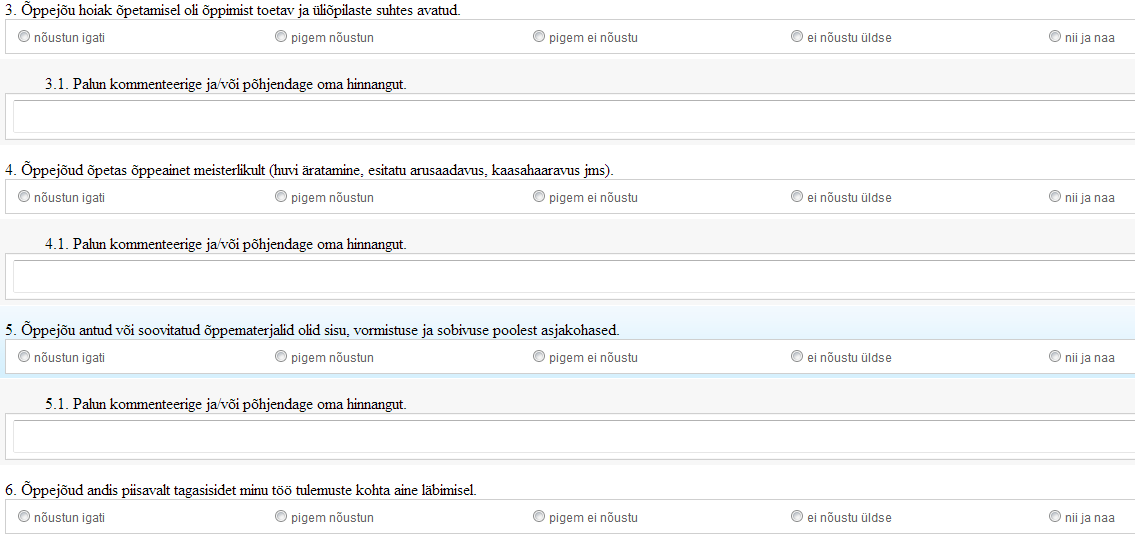
\includegraphics[width=0.8\textwidth]{ois_tagasiside_toodeldud.png}
\caption{Näide Tartu \"Ulikooli õppeinfo s\"usteemi tagasiside ankeedist, kus rakendatakse Likerti skaalat \cite{UT}}
\label{likert1}
\end{figure}

\begin{figure}[H]
\centering
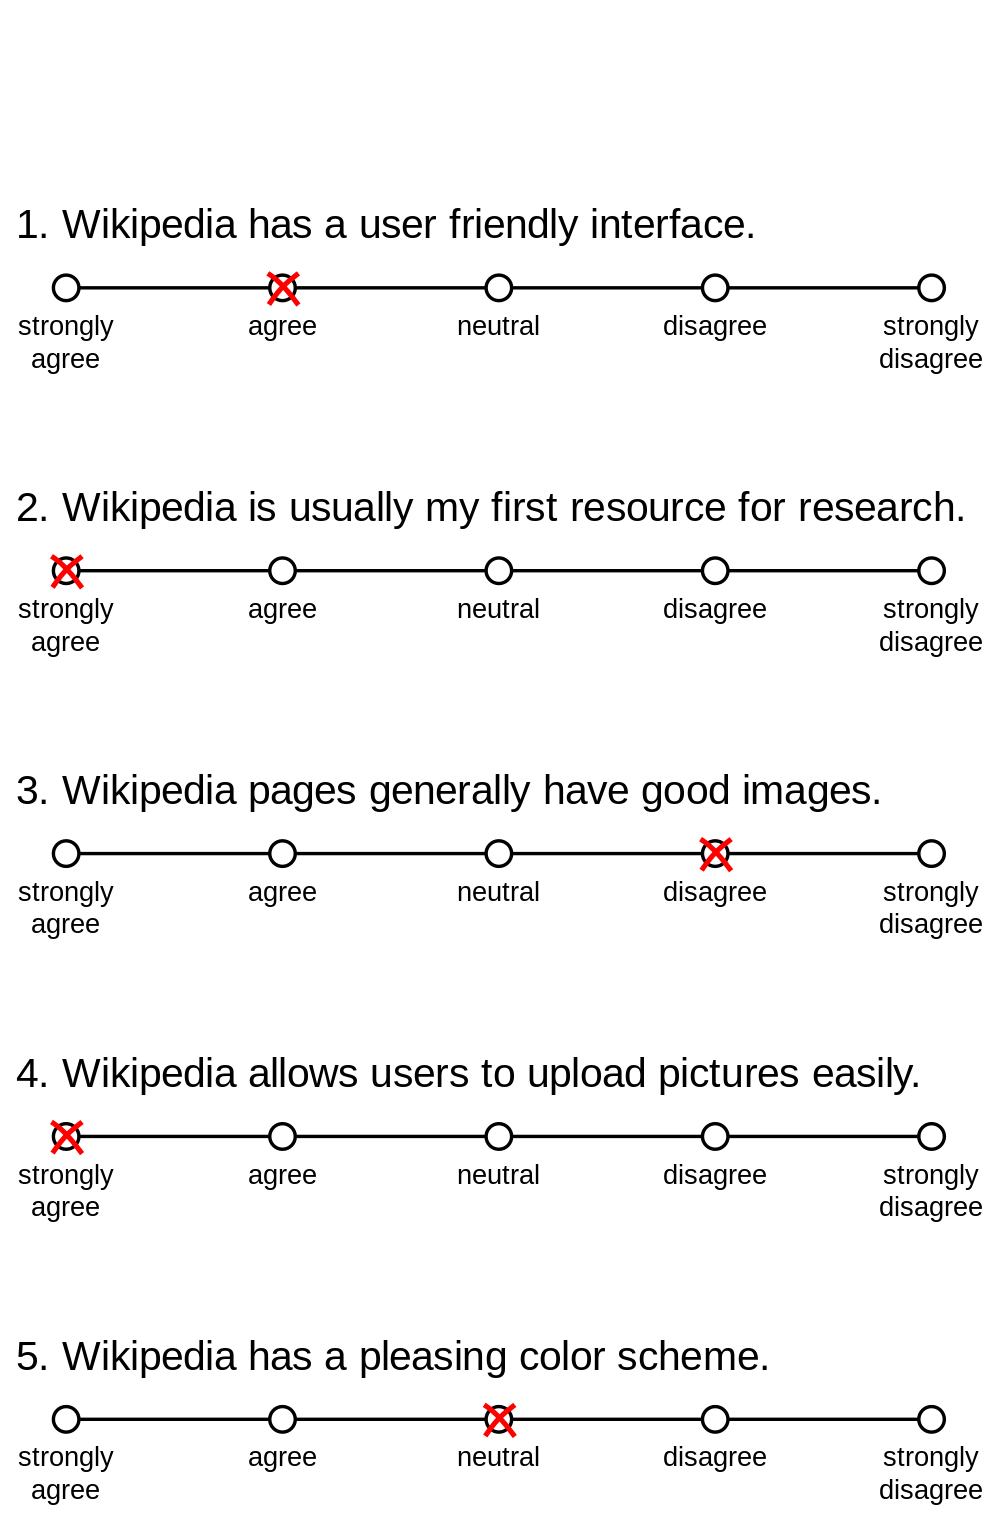
\includegraphics[width=0.5\textwidth, height = 0.7\textwidth]{Example_Likert_Scale.png}
\caption{Näide k\"usimustikust, kus rakendatud Likerti skaalat, k\"usimused on paigutatud nende järjestikulisus rõhutamiseks teljele\cite{Smith}}
\label{likert2}
\end{figure}



\pagebreak
\bibliography{mata_baka}{}
\bibliographystyle{plain}


\end{document}